\documentclass{article}
\usepackage{tikz}
\usetikzlibrary{calc}

\newcommand{\square}[1]{\pgfmathparse{#1*#1}\pgfmathresult}
\newcommand{\half}[1]{\pgfmathparse{#1/2.}\pgfmathresult}

\begin{document}
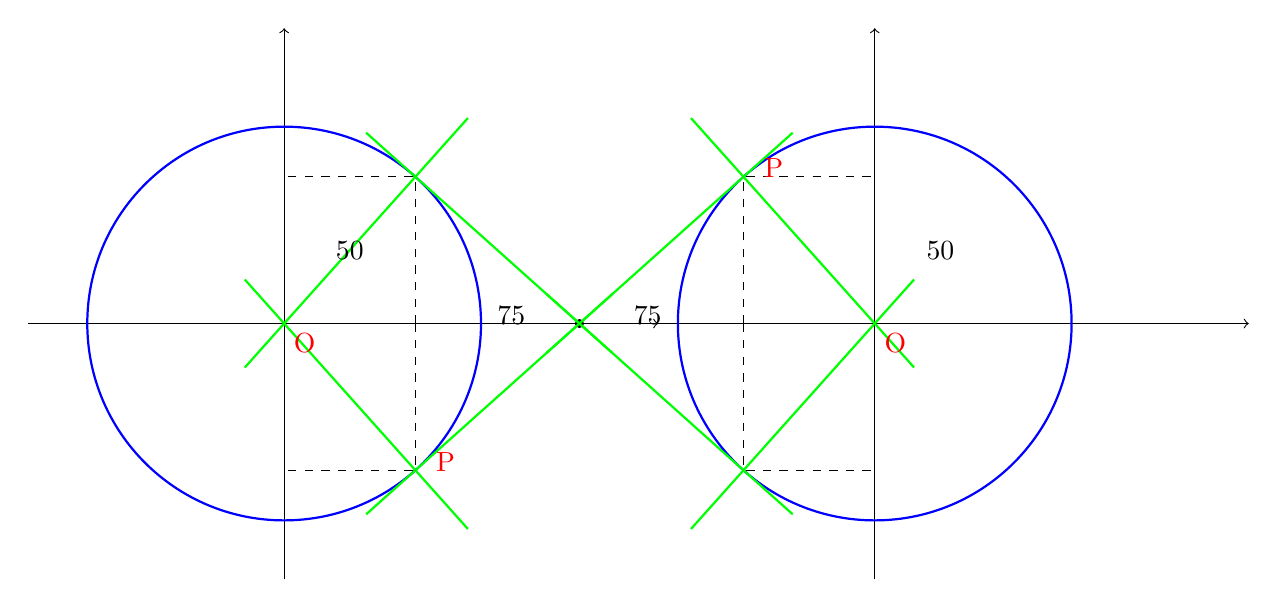
\begin{tikzpicture}[dot/.style={circle,draw=black, fill,inner sep=1pt},scale=0.05]
  \def\shft{150cm}
  \def\r{50} % radius
  \def\q{75} % distance center-external point q = |OQ|
\pgfmathsetmacro\x{{{\r^2/\q}}};
\pgfmathsetmacro\y{{{{\r*sqrt(1.-(\r/\q)^2}}}};
% \def\x{{\r^2/\q}} % Q x coordinate
% \def\y{-{\r*sqrt(1.-(\r/\q)^2}} % Q y coordinate
  \coordinate (O) at (0,0); % circle center O
  \coordinate (Q) at (\q,0); % external point Q
  \coordinate (P) at (\x,-\y); % point of tangency, P
  \draw[->] (0,-1.3*\r) -- (0,1.5*\r);
  \draw[->] (-1.3*\r,0) -- (\q+0.4*\r,0);
  \draw[dashed] (\x,0) |- (0,-\y);
  \draw[blue,thick] (O) circle(\r);
  \draw[green,thick] ($(Q)!-0.2!(P)$) -- ($(Q)!1.3!(P)$);
  \draw[green,thick] ($(O)!-0.3!(P)$) -- ($(O)!1.4!(P)$);
  \fill[red] (O) circle(0.05) node[below right] {O};
% \fill[red] (Q) circle(0.05) node[below left] {Q};
% \fill[red] (Q) circle(0.05) {};
% \draw[red] at (\q,0) circle(0.05) {};
  \node[dot] at (\q,0){};
  \fill[red] (P) circle(0.05) node[above=3,right=4] {P};

  \coordinate (P) at (\x,\y); % point of tangency, P
  \draw[dashed] (\x,0) |- (0,\y);
  \draw[green,thick] ($(Q)!-0.2!(P)$) -- ($(Q)!1.3!(P)$);
  \draw[green,thick] ($(O)!-0.3!(P)$) -- ($(O)!1.4!(P)$);

  \pgfmathsetmacro\hx{{\x/2.}};
  \pgfmathsetmacro\hy{\y/2.};
  \node (QQ) at ({\q/1.3},2)    {\q};

  \node (zzz) at (\hx,\hy) {\r};

\begin{scope}[xshift=\shft]
  \def\r{50} % radius
  \def\q{75} % distance center-external point q = |OQ|
  \pgfmathsetmacro\x{{{\r^2/\q}}};
  \pgfmathsetmacro\y{{{\r*sqrt(1.-(\r/\q)^2}}};
  \coordinate (O) at (0,0); % circle center O
  \coordinate (Q) at (-\q,0); % external point Q
  \coordinate (P) at (-\x,\y); % point of tangency, P
  \draw[->] (0,-1.3*\r) -- (0,1.5*\r);
  \draw[->] (-1.3*\r,0) -- (\q+0.4*\r,0);
  \draw[dashed] (-\x,0) |- (0,\y);
  \draw[blue,thick] (O) circle(\r);
  \draw[green,thick] ($(Q)!-0.2!(P)$) -- ($(Q)!1.3!(P)$);
  \draw[green,thick] ($(O)!-0.3!(P)$) -- ($(O)!1.4!(P)$);
  \fill[red] (O) circle(0.05) node[below right] {O};
% \fill[red] (Q) circle(0.05) node[below left] {Q};
  \fill[red] (P) circle(0.05) node[above=3,right=4] {P};

 \coordinate (P) at (-\x,-\y);
 \draw[dashed] (-\x,0) |- (0,-\y);
 \draw[green,thick] ($(Q)!-0.2!(P)$) -- ($(Q)!1.3!(P)$);
 \draw[green,thick] ($(O)!-0.3!(P)$) -- ($(O)!1.4!(P)$);

  \pgfmathsetmacro\hx{{\x/2.}};
  \pgfmathsetmacro\hy{\y/2.};
  \node (QQ) at ({-\q/1.3},2)    {\q};
  \node (zzz) at (\hx,\hy) {\r};
\end{scope}
\end{tikzpicture}

\end{document}
